\documentclass[]{article}
\usepackage{lmodern}
\usepackage{amssymb,amsmath}
\usepackage{ifxetex,ifluatex}
\usepackage{fixltx2e} % provides \textsubscript
\ifnum 0\ifxetex 1\fi\ifluatex 1\fi=0 % if pdftex
  \usepackage[T1]{fontenc}
  \usepackage[utf8]{inputenc}
\else % if luatex or xelatex
  \ifxetex
    \usepackage{mathspec}
  \else
    \usepackage{fontspec}
  \fi
  \defaultfontfeatures{Ligatures=TeX,Scale=MatchLowercase}
\fi
% use upquote if available, for straight quotes in verbatim environments
\IfFileExists{upquote.sty}{\usepackage{upquote}}{}
% use microtype if available
\IfFileExists{microtype.sty}{%
\usepackage{microtype}
\UseMicrotypeSet[protrusion]{basicmath} % disable protrusion for tt fonts
}{}
\usepackage[margin=1in]{geometry}
\usepackage{hyperref}
\hypersetup{unicode=true,
            pdfborder={0 0 0},
            breaklinks=true}
\urlstyle{same}  % don't use monospace font for urls
\usepackage{color}
\usepackage{fancyvrb}
\newcommand{\VerbBar}{|}
\newcommand{\VERB}{\Verb[commandchars=\\\{\}]}
\DefineVerbatimEnvironment{Highlighting}{Verbatim}{commandchars=\\\{\}}
% Add ',fontsize=\small' for more characters per line
\usepackage{framed}
\definecolor{shadecolor}{RGB}{248,248,248}
\newenvironment{Shaded}{\begin{snugshade}}{\end{snugshade}}
\newcommand{\KeywordTok}[1]{\textcolor[rgb]{0.13,0.29,0.53}{\textbf{#1}}}
\newcommand{\DataTypeTok}[1]{\textcolor[rgb]{0.13,0.29,0.53}{#1}}
\newcommand{\DecValTok}[1]{\textcolor[rgb]{0.00,0.00,0.81}{#1}}
\newcommand{\BaseNTok}[1]{\textcolor[rgb]{0.00,0.00,0.81}{#1}}
\newcommand{\FloatTok}[1]{\textcolor[rgb]{0.00,0.00,0.81}{#1}}
\newcommand{\ConstantTok}[1]{\textcolor[rgb]{0.00,0.00,0.00}{#1}}
\newcommand{\CharTok}[1]{\textcolor[rgb]{0.31,0.60,0.02}{#1}}
\newcommand{\SpecialCharTok}[1]{\textcolor[rgb]{0.00,0.00,0.00}{#1}}
\newcommand{\StringTok}[1]{\textcolor[rgb]{0.31,0.60,0.02}{#1}}
\newcommand{\VerbatimStringTok}[1]{\textcolor[rgb]{0.31,0.60,0.02}{#1}}
\newcommand{\SpecialStringTok}[1]{\textcolor[rgb]{0.31,0.60,0.02}{#1}}
\newcommand{\ImportTok}[1]{#1}
\newcommand{\CommentTok}[1]{\textcolor[rgb]{0.56,0.35,0.01}{\textit{#1}}}
\newcommand{\DocumentationTok}[1]{\textcolor[rgb]{0.56,0.35,0.01}{\textbf{\textit{#1}}}}
\newcommand{\AnnotationTok}[1]{\textcolor[rgb]{0.56,0.35,0.01}{\textbf{\textit{#1}}}}
\newcommand{\CommentVarTok}[1]{\textcolor[rgb]{0.56,0.35,0.01}{\textbf{\textit{#1}}}}
\newcommand{\OtherTok}[1]{\textcolor[rgb]{0.56,0.35,0.01}{#1}}
\newcommand{\FunctionTok}[1]{\textcolor[rgb]{0.00,0.00,0.00}{#1}}
\newcommand{\VariableTok}[1]{\textcolor[rgb]{0.00,0.00,0.00}{#1}}
\newcommand{\ControlFlowTok}[1]{\textcolor[rgb]{0.13,0.29,0.53}{\textbf{#1}}}
\newcommand{\OperatorTok}[1]{\textcolor[rgb]{0.81,0.36,0.00}{\textbf{#1}}}
\newcommand{\BuiltInTok}[1]{#1}
\newcommand{\ExtensionTok}[1]{#1}
\newcommand{\PreprocessorTok}[1]{\textcolor[rgb]{0.56,0.35,0.01}{\textit{#1}}}
\newcommand{\AttributeTok}[1]{\textcolor[rgb]{0.77,0.63,0.00}{#1}}
\newcommand{\RegionMarkerTok}[1]{#1}
\newcommand{\InformationTok}[1]{\textcolor[rgb]{0.56,0.35,0.01}{\textbf{\textit{#1}}}}
\newcommand{\WarningTok}[1]{\textcolor[rgb]{0.56,0.35,0.01}{\textbf{\textit{#1}}}}
\newcommand{\AlertTok}[1]{\textcolor[rgb]{0.94,0.16,0.16}{#1}}
\newcommand{\ErrorTok}[1]{\textcolor[rgb]{0.64,0.00,0.00}{\textbf{#1}}}
\newcommand{\NormalTok}[1]{#1}
\usepackage{graphicx,grffile}
\makeatletter
\def\maxwidth{\ifdim\Gin@nat@width>\linewidth\linewidth\else\Gin@nat@width\fi}
\def\maxheight{\ifdim\Gin@nat@height>\textheight\textheight\else\Gin@nat@height\fi}
\makeatother
% Scale images if necessary, so that they will not overflow the page
% margins by default, and it is still possible to overwrite the defaults
% using explicit options in \includegraphics[width, height, ...]{}
\setkeys{Gin}{width=\maxwidth,height=\maxheight,keepaspectratio}
\IfFileExists{parskip.sty}{%
\usepackage{parskip}
}{% else
\setlength{\parindent}{0pt}
\setlength{\parskip}{6pt plus 2pt minus 1pt}
}
\setlength{\emergencystretch}{3em}  % prevent overfull lines
\providecommand{\tightlist}{%
  \setlength{\itemsep}{0pt}\setlength{\parskip}{0pt}}
\setcounter{secnumdepth}{0}
% Redefines (sub)paragraphs to behave more like sections
\ifx\paragraph\undefined\else
\let\oldparagraph\paragraph
\renewcommand{\paragraph}[1]{\oldparagraph{#1}\mbox{}}
\fi
\ifx\subparagraph\undefined\else
\let\oldsubparagraph\subparagraph
\renewcommand{\subparagraph}[1]{\oldsubparagraph{#1}\mbox{}}
\fi

%%% Use protect on footnotes to avoid problems with footnotes in titles
\let\rmarkdownfootnote\footnote%
\def\footnote{\protect\rmarkdownfootnote}

%%% Change title format to be more compact
\usepackage{titling}

% Create subtitle command for use in maketitle
\newcommand{\subtitle}[1]{
  \posttitle{
    \begin{center}\large#1\end{center}
    }
}

\setlength{\droptitle}{-2em}

  \title{}
    \pretitle{\vspace{\droptitle}}
  \posttitle{}
    \author{}
    \preauthor{}\postauthor{}
    \date{}
    \predate{}\postdate{}
  

\begin{document}

\begin{Shaded}
\begin{Highlighting}[]
\NormalTok{knitr}\OperatorTok{::}\NormalTok{opts_chunk}\OperatorTok{$}\KeywordTok{set}\NormalTok{(}\DataTypeTok{echo =} \OtherTok{TRUE}\NormalTok{)}
\NormalTok{nsims <-}\StringTok{ }\DecValTok{100000} \CommentTok{#set number of simulations}
\KeywordTok{library}\NormalTok{(mvtnorm, }\DataTypeTok{quietly =} \OtherTok{TRUE}\NormalTok{)}
\KeywordTok{library}\NormalTok{(MASS, }\DataTypeTok{quietly =} \OtherTok{TRUE}\NormalTok{)}
\KeywordTok{library}\NormalTok{(afex, }\DataTypeTok{quietly =} \OtherTok{TRUE}\NormalTok{)}
\KeywordTok{library}\NormalTok{(emmeans, }\DataTypeTok{quietly =} \OtherTok{TRUE}\NormalTok{)}
\KeywordTok{library}\NormalTok{(ggplot2, }\DataTypeTok{quietly =} \OtherTok{TRUE}\NormalTok{)}
\KeywordTok{library}\NormalTok{(gridExtra, }\DataTypeTok{quietly =} \OtherTok{TRUE}\NormalTok{)}
\KeywordTok{library}\NormalTok{(reshape2, }\DataTypeTok{quietly =} \OtherTok{TRUE}\NormalTok{)}
\KeywordTok{library}\NormalTok{(pwr, }\DataTypeTok{quietly =} \OtherTok{TRUE}\NormalTok{)}

\CommentTok{# Install functions from GitHub by running the code below:}
\KeywordTok{source}\NormalTok{(}\StringTok{"https://raw.githubusercontent.com/Lakens/ANOVA_power_simulation/master/ANOVA_design.R"}\NormalTok{)}
\KeywordTok{source}\NormalTok{(}\StringTok{"https://raw.githubusercontent.com/Lakens/ANOVA_power_simulation/master/ANOVA_power.R"}\NormalTok{)}
\KeywordTok{source}\NormalTok{(}\StringTok{"https://raw.githubusercontent.com/Lakens/ANOVA_power_simulation/master/helper_functions/power_oneway_between.R"}\NormalTok{)}
\KeywordTok{source}\NormalTok{(}\StringTok{"https://raw.githubusercontent.com/Lakens/ANOVA_power_simulation/master/helper_functions/power_oneway_within.R"}\NormalTok{)}
\KeywordTok{source}\NormalTok{(}\StringTok{"https://raw.githubusercontent.com/Lakens/ANOVA_power_simulation/master/helper_functions/power_twoway_between.R"}\NormalTok{)}
\KeywordTok{source}\NormalTok{(}\StringTok{"https://raw.githubusercontent.com/Lakens/ANOVA_power_simulation/master/helper_functions/power_2x2_within.R"}\NormalTok{)}
\KeywordTok{source}\NormalTok{(}\StringTok{"https://raw.githubusercontent.com/Lakens/ANOVA_power_simulation/master/helper_functions/plot_power_oneway_between.R"}\NormalTok{)}
\KeywordTok{source}\NormalTok{(}\StringTok{"https://raw.githubusercontent.com/Lakens/ANOVA_power_simulation/master/helper_functions/plot_power_oneway_within.R"}\NormalTok{)}
\KeywordTok{source}\NormalTok{(}\StringTok{"https://raw.githubusercontent.com/Lakens/ANOVA_power_simulation/master/helper_functions/plot_power_twoway_between.R"}\NormalTok{)}
\KeywordTok{source}\NormalTok{(}\StringTok{"https://raw.githubusercontent.com/Lakens/ANOVA_power_simulation/master/helper_functions/plot_power_2x2_within.R"}\NormalTok{)}
\end{Highlighting}
\end{Shaded}

\subsection{Power for Three-way
Interactions}\label{power-for-three-way-interactions}

There are almost no software solutions that allow researchers to perform
power anaysis for more complex designs. Through simulation, it is
relatively straightforward to examine the power for designs with
multiple factors with many levels.

Let's start with a 2x2x2 between subjects design. We collect 50
participants in each between participant condition (so 400 participants
in total - 50x2x2x2).

\begin{Shaded}
\begin{Highlighting}[]
\NormalTok{string <-}\StringTok{ "2b*2b*2b"}
\NormalTok{n <-}\StringTok{ }\DecValTok{50}
\NormalTok{mu <-}\StringTok{ }\KeywordTok{c}\NormalTok{(}\DecValTok{1}\NormalTok{, }\DecValTok{1}\NormalTok{, }\DecValTok{6}\NormalTok{, }\DecValTok{1}\NormalTok{, }\DecValTok{6}\NormalTok{, }\DecValTok{6}\NormalTok{, }\DecValTok{1}\NormalTok{, }\DecValTok{6}\NormalTok{) }
\NormalTok{sd <-}\StringTok{ }\DecValTok{10}
\NormalTok{r <-}\StringTok{ }\FloatTok{0.0}
\NormalTok{labelnames <-}\StringTok{ }\KeywordTok{c}\NormalTok{(}\StringTok{"Size"}\NormalTok{, }\StringTok{"big"}\NormalTok{, }\StringTok{"small"}\NormalTok{, }\StringTok{"Color"}\NormalTok{, }\StringTok{"green"}\NormalTok{, }\StringTok{"red"}\NormalTok{, }
                \StringTok{"CognitiveLoad"}\NormalTok{, }\StringTok{"present"}\NormalTok{, }\StringTok{"absent"}\NormalTok{) }\CommentTok{#}

\NormalTok{design_result <-}\StringTok{ }\KeywordTok{ANOVA_design}\NormalTok{(}\DataTypeTok{string =}\NormalTok{ string,}
                   \DataTypeTok{n =}\NormalTok{ n, }
                   \DataTypeTok{mu =}\NormalTok{ mu, }
                   \DataTypeTok{sd =}\NormalTok{ sd, }
                   \DataTypeTok{labelnames =}\NormalTok{ labelnames)}
\end{Highlighting}
\end{Shaded}

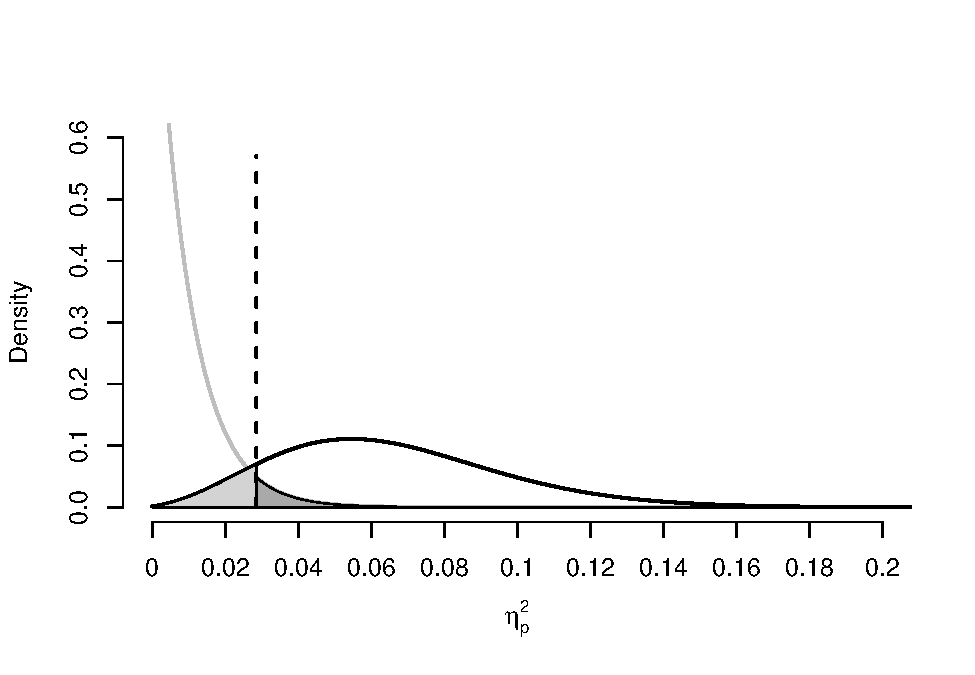
\includegraphics{4.6_threeway_interactions_files/figure-latex/unnamed-chunk-1-1.pdf}

\begin{Shaded}
\begin{Highlighting}[]
\CommentTok{# Power for the given N in the design_result}
\KeywordTok{ANOVA_power}\NormalTok{(design_result, }\DataTypeTok{nsims =}\NormalTok{ nsims)}
\end{Highlighting}
\end{Shaded}

\begin{verbatim}
## Power and Effect sizes for ANOVA tests
##                                 power effect size
## anova_Size                     70.179      0.0156
## anova_Color                     4.969      0.0012
## anova_CognitiveLoad             4.948      0.0012
## anova_Size:Color               70.192      0.0157
## anova_Size:CognitiveLoad       70.369      0.0157
## anova_Color:CognitiveLoad       5.036      0.0012
## anova_Size:Color:CognitiveLoad 70.605      0.0158
## 
## Power and Effect sizes for contrasts
##                                                                                             power effect size
## p_Size_big_Color_green_CognitiveLoad_present_Size_big_Color_green_CognitiveLoad_absent      4.963     -0.0007
## p_Size_big_Color_green_CognitiveLoad_present_Size_big_Color_red_CognitiveLoad_present      69.630      0.5035
## p_Size_big_Color_green_CognitiveLoad_present_Size_big_Color_red_CognitiveLoad_absent        4.960     -0.0004
## p_Size_big_Color_green_CognitiveLoad_present_Size_small_Color_green_CognitiveLoad_present  69.727      0.5032
## p_Size_big_Color_green_CognitiveLoad_present_Size_small_Color_green_CognitiveLoad_absent   69.399      0.5024
## p_Size_big_Color_green_CognitiveLoad_present_Size_small_Color_red_CognitiveLoad_present     5.022     -0.0011
## p_Size_big_Color_green_CognitiveLoad_present_Size_small_Color_red_CognitiveLoad_absent     69.697      0.5035
## p_Size_big_Color_green_CognitiveLoad_absent_Size_big_Color_red_CognitiveLoad_present       69.661      0.5043
## p_Size_big_Color_green_CognitiveLoad_absent_Size_big_Color_red_CognitiveLoad_absent         4.906      0.0003
## p_Size_big_Color_green_CognitiveLoad_absent_Size_small_Color_green_CognitiveLoad_present   69.715      0.5040
## p_Size_big_Color_green_CognitiveLoad_absent_Size_small_Color_green_CognitiveLoad_absent    69.442      0.5031
## p_Size_big_Color_green_CognitiveLoad_absent_Size_small_Color_red_CognitiveLoad_present      4.855     -0.0004
## p_Size_big_Color_green_CognitiveLoad_absent_Size_small_Color_red_CognitiveLoad_absent      69.644      0.5043
## p_Size_big_Color_red_CognitiveLoad_present_Size_big_Color_red_CognitiveLoad_absent         69.719     -0.5041
## p_Size_big_Color_red_CognitiveLoad_present_Size_small_Color_green_CognitiveLoad_present     5.103     -0.0004
## p_Size_big_Color_red_CognitiveLoad_present_Size_small_Color_green_CognitiveLoad_absent      4.987     -0.0012
## p_Size_big_Color_red_CognitiveLoad_present_Size_small_Color_red_CognitiveLoad_present      69.737     -0.5046
## p_Size_big_Color_red_CognitiveLoad_present_Size_small_Color_red_CognitiveLoad_absent        4.930     -0.0001
## p_Size_big_Color_red_CognitiveLoad_absent_Size_small_Color_green_CognitiveLoad_present     69.864      0.5037
## p_Size_big_Color_red_CognitiveLoad_absent_Size_small_Color_green_CognitiveLoad_absent      69.432      0.5030
## p_Size_big_Color_red_CognitiveLoad_absent_Size_small_Color_red_CognitiveLoad_present        4.886     -0.0007
## p_Size_big_Color_red_CognitiveLoad_absent_Size_small_Color_red_CognitiveLoad_absent        69.711      0.5041
## p_Size_small_Color_green_CognitiveLoad_present_Size_small_Color_green_CognitiveLoad_absent  5.115     -0.0009
## p_Size_small_Color_green_CognitiveLoad_present_Size_small_Color_red_CognitiveLoad_present  69.814     -0.5042
## p_Size_small_Color_green_CognitiveLoad_present_Size_small_Color_red_CognitiveLoad_absent    5.018      0.0004
## p_Size_small_Color_green_CognitiveLoad_absent_Size_small_Color_red_CognitiveLoad_present   69.716     -0.5035
## p_Size_small_Color_green_CognitiveLoad_absent_Size_small_Color_red_CognitiveLoad_absent     5.099      0.0013
## p_Size_small_Color_red_CognitiveLoad_present_Size_small_Color_red_CognitiveLoad_absent     69.641      0.5046
\end{verbatim}

A Three-Way ANOVA builds on the same principles as a One\_Way ANOVA. We
look at whether the differences between groups are large, compared to
the standard deviation. For the main effects we simply have 2 groups of
200 participants, and 2 means. If the population standard deviations are
identical across groups, this is not in any way different from a One-Way
ANOVA. Indeed, we can show this by simulating a One-Way ANOVA, where
instead of 8 conditions, we have two conditions, and we average over the
4 groups of the other two factors. For example, for the main effect of
size above:

\begin{Shaded}
\begin{Highlighting}[]
\NormalTok{string <-}\StringTok{ "2b"}
\NormalTok{n <-}\StringTok{ }\DecValTok{200}
\NormalTok{mu <-}\StringTok{ }\KeywordTok{c}\NormalTok{(}\KeywordTok{mean}\NormalTok{(}\KeywordTok{c}\NormalTok{(}\DecValTok{1}\NormalTok{, }\DecValTok{1}\NormalTok{, }\DecValTok{6}\NormalTok{, }\DecValTok{1}\NormalTok{)), }\KeywordTok{mean}\NormalTok{(}\KeywordTok{c}\NormalTok{(}\DecValTok{6}\NormalTok{, }\DecValTok{6}\NormalTok{, }\DecValTok{1}\NormalTok{, }\DecValTok{6}\NormalTok{)))}
\NormalTok{sd <-}\StringTok{ }\DecValTok{10}
\NormalTok{labelnames <-}\StringTok{ }\KeywordTok{c}\NormalTok{(}\StringTok{"Size"}\NormalTok{, }\StringTok{"big"}\NormalTok{, }\StringTok{"small"}\NormalTok{)}

\NormalTok{design_result <-}\StringTok{ }\KeywordTok{ANOVA_design}\NormalTok{(}\DataTypeTok{string =}\NormalTok{ string,}
                   \DataTypeTok{n =}\NormalTok{ n, }
                   \DataTypeTok{mu =}\NormalTok{ mu, }
                   \DataTypeTok{sd =}\NormalTok{ sd, }
                   \DataTypeTok{labelnames =}\NormalTok{ labelnames)}
\end{Highlighting}
\end{Shaded}

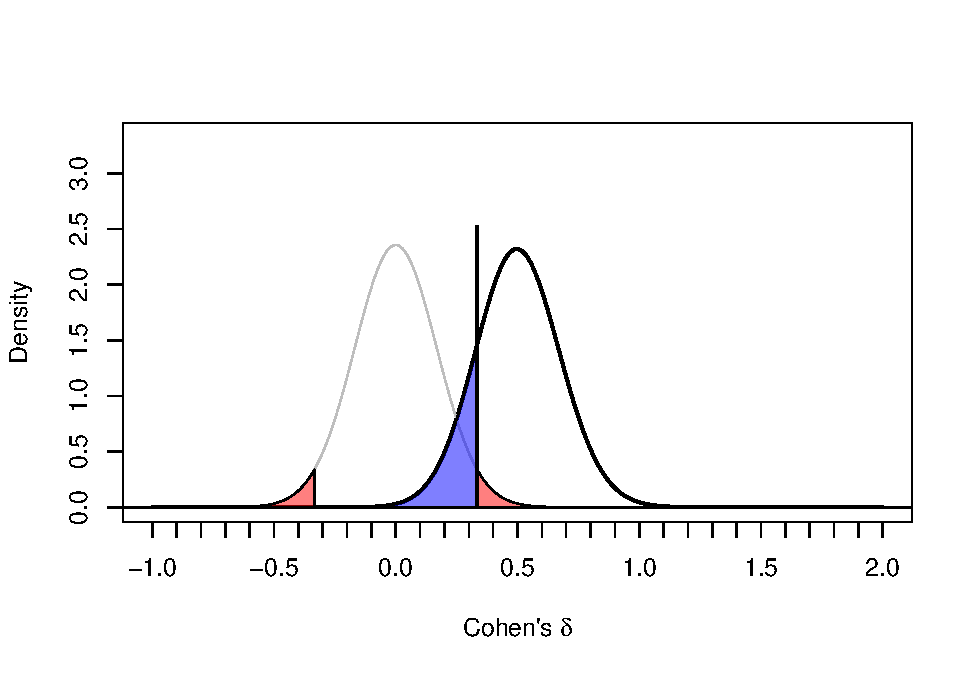
\includegraphics{4.6_threeway_interactions_files/figure-latex/unnamed-chunk-2-1.pdf}

\begin{Shaded}
\begin{Highlighting}[]
\CommentTok{# Power based on simulations}
\KeywordTok{ANOVA_power}\NormalTok{(design_result, }\DataTypeTok{nsims =}\NormalTok{ nsims)}
\end{Highlighting}
\end{Shaded}

\begin{verbatim}
## Power and Effect sizes for ANOVA tests
##             power effect size
## anova_Size 70.655      0.0156
## 
## Power and Effect sizes for contrasts
##                        power effect size
## p_Size_big_Size_small 70.655      0.2513
\end{verbatim}

\begin{Shaded}
\begin{Highlighting}[]
\CommentTok{# Power based on analytical solution}
\KeywordTok{power_oneway_between}\NormalTok{(design_result)}\OperatorTok{$}\NormalTok{power }\CommentTok{#using default alpha level of .05}
\end{Highlighting}
\end{Shaded}

\begin{verbatim}
## [1] 0.7033333
\end{verbatim}

Similarly, we can create a 2 factor design where we average over the
third factor, and recreate the power analysis for the Two-Way
interaction. For example, we can group over the Cognitive Load
condition, and look at the Size by Color Interaction:

\begin{Shaded}
\begin{Highlighting}[]
\NormalTok{string <-}\StringTok{ "2b*2b"}
\NormalTok{n <-}\StringTok{ }\DecValTok{100}
\NormalTok{mu <-}\StringTok{ }\KeywordTok{c}\NormalTok{(}\KeywordTok{mean}\NormalTok{(}\KeywordTok{c}\NormalTok{(}\DecValTok{1}\NormalTok{, }\DecValTok{1}\NormalTok{)), }\KeywordTok{mean}\NormalTok{(}\KeywordTok{c}\NormalTok{(}\DecValTok{6}\NormalTok{, }\DecValTok{1}\NormalTok{)), }\KeywordTok{mean}\NormalTok{(}\KeywordTok{c}\NormalTok{(}\DecValTok{6}\NormalTok{, }\DecValTok{6}\NormalTok{)), }\KeywordTok{mean}\NormalTok{(}\KeywordTok{c}\NormalTok{(}\DecValTok{1}\NormalTok{, }\DecValTok{6}\NormalTok{)))}
\NormalTok{sd <-}\StringTok{ }\DecValTok{10}
\NormalTok{labelnames <-}\StringTok{ }\KeywordTok{c}\NormalTok{(}\StringTok{"Size"}\NormalTok{, }\StringTok{"big"}\NormalTok{, }\StringTok{"small"}\NormalTok{, }\StringTok{"Color"}\NormalTok{, }\StringTok{"green"}\NormalTok{, }\StringTok{"red"}\NormalTok{)}

\NormalTok{design_result <-}\StringTok{ }\KeywordTok{ANOVA_design}\NormalTok{(}\DataTypeTok{string =}\NormalTok{ string,}
                   \DataTypeTok{n =}\NormalTok{ n, }
                   \DataTypeTok{mu =}\NormalTok{ mu, }
                   \DataTypeTok{sd =}\NormalTok{ sd, }
                   \DataTypeTok{labelnames =}\NormalTok{ labelnames)}
\end{Highlighting}
\end{Shaded}

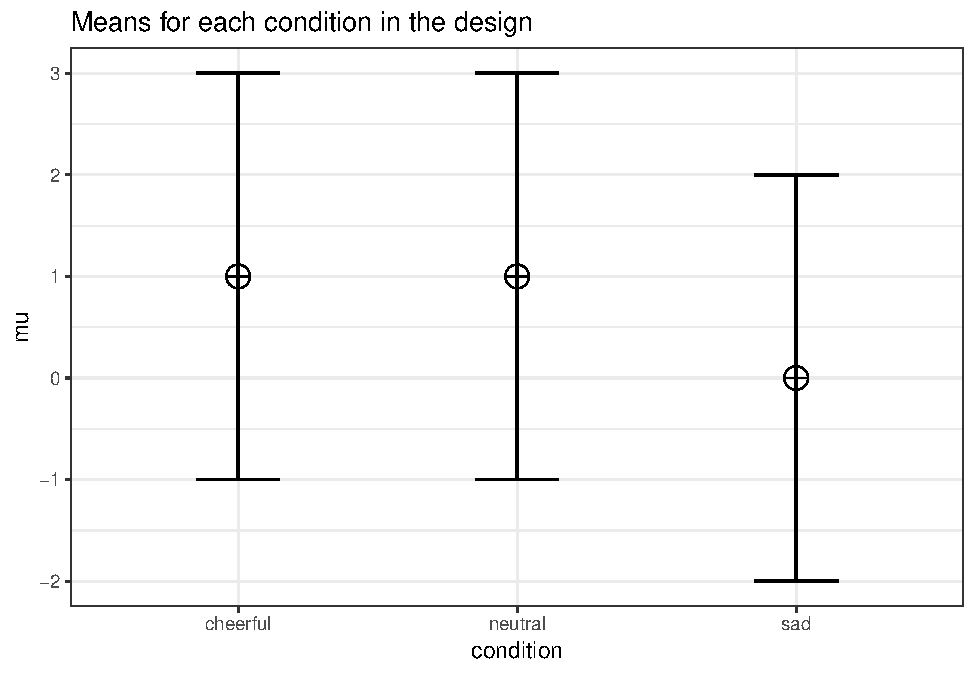
\includegraphics{4.6_threeway_interactions_files/figure-latex/unnamed-chunk-3-1.pdf}

\begin{Shaded}
\begin{Highlighting}[]
\CommentTok{# Power based on simulations}
\KeywordTok{ANOVA_power}\NormalTok{(design_result, }\DataTypeTok{nsims =}\NormalTok{ nsims)}
\end{Highlighting}
\end{Shaded}

\begin{verbatim}
## Power and Effect sizes for ANOVA tests
##                   power effect size
## anova_Size       70.326      0.0156
## anova_Color       5.047      0.0012
## anova_Size:Color 70.518      0.0157
## 
## Power and Effect sizes for contrasts
##                                                power effect size
## p_Size_big_Color_green_Size_big_Color_red     42.250      0.2516
## p_Size_big_Color_green_Size_small_Color_green 93.984      0.5025
## p_Size_big_Color_green_Size_small_Color_red   42.146      0.2511
## p_Size_big_Color_red_Size_small_Color_green   41.951      0.2509
## p_Size_big_Color_red_Size_small_Color_red      5.102     -0.0006
## p_Size_small_Color_green_Size_small_Color_red 42.146     -0.2514
\end{verbatim}

\begin{Shaded}
\begin{Highlighting}[]
\CommentTok{# Power based on analytical solution}
\NormalTok{power_res <-}\StringTok{ }\KeywordTok{power_twoway_between}\NormalTok{(design_result) }\CommentTok{#using default alpha level of .05}

\NormalTok{power_res}\OperatorTok{$}\NormalTok{power_A}
\end{Highlighting}
\end{Shaded}

\begin{verbatim}
## [1] 0.7033228
\end{verbatim}

\begin{Shaded}
\begin{Highlighting}[]
\NormalTok{power_res}\OperatorTok{$}\NormalTok{power_B}
\end{Highlighting}
\end{Shaded}

\begin{verbatim}
## [1] 0.05
\end{verbatim}

\begin{Shaded}
\begin{Highlighting}[]
\NormalTok{power_res}\OperatorTok{$}\NormalTok{power_AB}
\end{Highlighting}
\end{Shaded}

\begin{verbatim}
## [1] 0.7033228
\end{verbatim}


\end{document}
